\documentclass[conference,onecolumn]{IEEEtran}

\usepackage{amssymb,amsthm,amsmath}
\usepackage{microtype}
%\usepackage{enumitem}
\usepackage[T1]{fontenc}
\usepackage{textcomp}
\usepackage{mathtools}

% Sorts citations; e.g. [1], [2], [5]--[7]
%\usepackage{cite}

% More reference handling options
%\usepackage{natbib}\renewcommand\bibfont{\footnotesize}

\usepackage{mllequiv,willemtools}

\graphicspath{{../notes/}}

\let\alt=\underline

\shortJournalNames
\makeTheoremDefs


\author{
  \IEEEauthorblockN{Willem Heijltjes}
  \IEEEauthorblockA{
  		University of Bath
	\\	Claverton Down
	\\	Bath BA2~7AY
	\\	w.b.heijltjes@bath.ac.uk
	}
\and
  \IEEEauthorblockN{Robin Houston}
  \IEEEauthorblockA{
		Kiln Enterprises
	\\	robin.houston@gmail.com	
	}
}

%\title{The proof equivalence problem for multiplicative linear logic is \textsc{pspace}-complete}

%\title{Proof equivalence in MLL is \textsc{pspace}-complete}

\title{No proof nets for MLL with units\\[5pt]\Large Proof equivalence in MLL is \textsc{pspace}-complete}

%============================================================

\begin{document}

\maketitle

\begin{abstract}
MLL proof equivalence is the problem of deciding whether two proofs in multiplicative linear logic are related by a series of inference permutations.
%
It is also known as the word problem for $*$-autonomous categories.
%
Previous work has shown the problem to be equivalent to a rewiring problem on proof nets, which are not canonical for full MLL due to the presence of the two units.
%
Drawing from recent work on reconfiguration problems, in this paper it is shown that MLL proof equivalence is PSPACE-complete, using a reduction from Nondeterministic Constraint Logic.
%
An important consequence of the result is that the existence of a satisfactory notion of proof nets for MLL with units is ruled out (under current complexity assumptions).
\end{abstract}


%------------------------------------------------------------

\section{Introduction}


%% STILL TO ADD:
%% - MLL proof equivalence is the word problem for *-autonomous categories
%% - IMLL proof equivalence is polynomial-time


An important element of the theory of linear logic \cite{Girard-1987} is the idea that proofs should be considered modulo the permutation of inferences.
%; that the chosen order of permutable inferences is inessential, or `bureaucracy'.
%contributes no essential proof content, and should be considered `bureaucracy'.
%
%The idea is supported by the categorical semantics of linear logic, in which proofs up to permutations denote the same morphism. 
%
\emph{Proof equivalence} is the problem of deciding whether two proofs are equal modulo permutations.


The proof equivalence problem is closely related to the notion of \emph{proof nets}.
%
These are canonical, geometric representations of proof that factor out permutations, so that proofs are equivalent if and only if they have the same underlying proof net.
%
Canonical proof nets have been found for several fragments of linear logic: the multipicative fragment without units \cite{Girard-1987,Danos-Regnier-1989}, the combined multiplicative-additive fragment without units \cite{Hughes-vanGlabbeek-2005}, and the additive fragment, including the additive units \cite{Heijltjes-2011}.
%
For the full multiplicative fragment, with units, several notions of proof net have been proposed \cite{BCST,Strassburger-lamarche-2004,HughesFreeStar}.
%
However, none is canonical, and whether a satisfactory notion of proof net can be found has remained an open question.



In this paper we establish that the proof equivalence problem for multiplicative linear logic with units is \textsc{pspace}-complete.
%
As a main corrolary, this effectively rules out the possibility of finding a satisfactory notion of proof net for this fragment.


% - - - - - - - - - - - - - - - - - - - - - - - - - - - - - -

\subsection*{Constraint logic and reconfiguration problems}

The proof of the \textsc{pspace}-completeness result relies on a polynomial reduction from %the configuration--to--configuration problem in
\emph{constraint logic}, a graphical formalism recently introduced as a uniform tool for use in complexity reductions \cite{Demaine-Hearn-2008}.
%
It consists of a simple graph rewriting mechanism, where weighted edges may be reversed as long as the given in-flow constraint for each vertex is satisfied, and asks whether two graphs are related in a series of valid rewriting steps.



Constraint logic belongs to a class of problems called \emph{reconfiguration problems} \cite{ReconfigurationProblems}: can one solution to a given problem be transformed into another by a series of elementary changes, while remaining valid throughout?
%
For example, for boolean satisfyability (SAT) the reconfiguration problem asks whether one satisfying assignment can be transformed into another by changing the value of one atomic formula at a time, without passing via a non-satisfying assignment.
%
It is not uncommon for an \textsc{np}-complete problem to have an associated reconfiguration problem that is \textsc{pspace}-complete \cite{ReconfigurationProblems}; one example is SAT-reconfiguration, which is \textsc{pspace}-complete.



MLL proof equivalence may be usefully classified as the reconfiguration problem associated with MLL proof search, which is \textsc{np}-complete \cite{Kanovich-1992}.




%------------------------------------------------------------

\section{MLL}



\begin{figure}[!b]
\quad\MLLrule b
\hfill\MLLrule 1
\hfill\MLLrule p
\hfill\MLLrule t
\quad
\caption{Inference rules for unit-only \MLL}
\label{fig:MLL}
\end{figure}


\begin{figure}[!tb]
\renewcommand\scalefactor{0.88}
\[
\begin{array}{@{}rcl@{}}
	\multicolumn{3}{@{}c@{}}{
		\vc{\scale{\MLLperm{bb1}}} ~\perm~ \vc{\scale{\MLLperm{bb2}}}
		\hfill
		\vc{\scale{\MLLperm{bp1}}} ~\perm~ \vc{\scale{\MLLperm{bp2}}}
	}
\\ \\[6pt]
	\multicolumn{3}{@{}c@{}}{
		\vc{\scale{\MLLperm{bt2}}} ~\perm~ \vc{\scale{\MLLperm{bt1}}}
								   ~\perm~ \vc{\scale{\MLLperm{bt3}}}
	}
\\ \\[6pt]
	\vc{\scale{\MLLperm{pp1}}} &\perm& \vc{\scale{\MLLperm{pp2}}}
\\ \\[6pt]
	\vc{\scale{\MLLperm{pt1}}} &\perm& \vc{\scale{\MLLperm{pt2}}}
\\ \\[6pt]
	\vc{\scale{\MLLperm{tt1}}} &\perm& \vc{\scale{\MLLperm{tt2}}}
\end{array}
\]
\caption{Permutations}
\label{fig:permutations}
\end{figure}





The formulae of unit-only multiplicative linear logic are given by the following grammar.
%
\setMidspace{5pt}
\[
	A,B,C \Coloneq \bot \Mid 1 \Mid A\parr B \Mid A\tn B
\]
%
The connectives $\tn$ and $\parr$ will be considered up to associativity, and \emph{duality} $\dual A$ is via DeMorgan.
%
A \emph{sequent} $\Gamma,\Delta$ will be a multiset of formulae.
%
Within a sequent, connectives and units will be \emph{named} with distinct elements from an arbitrary set of names, e.g.\
$\named a1\named b\parr\named c1,\named d\bot\named e\tn\named f\bot$.
%
This allows to 1) identify \emph{occurrences} of subformulae uniquely by the name of their root connective, e.g.\ as $\named bA$, 2) distinguish the two proofs of the above sequent while using standard multiset sequents, and 3) easily extract proof nets, as graphs using the names of connectives as vertices.
%
Names will mostly be left implicit.



Proofs are constructed from the inference rules in Figure~\ref{fig:MLL}, where the names of units and connectives are preserved through inferences.
%
Only cut-free proofs are considered, and no cut-rule is added.
%
\emph{Permutations} of inference rules are displayed in Figure~\ref{fig:permutations}; the symmetric variants of the last two permutations, \emph{par-tensor} and \emph{tensor-tensor}, have been omitted.



\begin{definition}
\label{def:equivalence}
%
\emph{Equivalence} of proofs $(\perm)$ in (cut-free, unit-only) multiplicative linear logic is the congruence generated by the permutations given in Figure~\ref{fig:permutations}.
%
\emph{\MLL\ proof equivalence} is the problem of deciding whether two given proofs are equivalent.
%
\end{definition}


% - - - - - - - - - - - - - - - - - - - - - - - - - - - - - -

\subsection*{Proof nets}

Proof nets provide a solution to proof equivalence for MLL$^-$ (MLL without units).
%
For full MLL, they reduce the proof equivalence problem to a simple rewiring relation \cite{HughesMLLProofNets}.


\begin{definition}
\label{def:proof nets}
%
For a sequent $\Gamma$,
\begin{itemize}

	\item
	a \emph{linking} $\links$ is a function from the names of $\bot$-subformulae to the names of $1$-subformulae,

	\item
	a \emph{switching graph} for $\links$ is an undirected graph over the names of $\Gamma$, with for every subformula $\named aA\named c\tn\named bB$ the edges $\edge ac$ and $\edge bc$, for every subformula $\named aA\named c\parr\named bB$ either the edge $\edge ac$ or the edge $\edge bc$, and for every subformula $\named a\bot$ the edge $\edge a{\links(a)}$,

 	\item
	a \emph{proof net} $\links$ or $(\Gamma,\links)$ is a linking $\links$ such that every switching graph is acyclic and connected.

\end{itemize}
\end{definition}


\noindent
An edge $\edge a{\links(a)}$ in a proof net or switching graph is called a \emph{link} or a \emph{jump}.



\begin{definition}
\label{def:proof net equivalence}
%
A \emph{permutation} $(\perm*)$ between proof nets is the redirection of exactly one link.
%
\emph{Equivalence} $(\perm)$ of proof nets over a sequent $\Gamma$ is the equivalence generated by permutations.
%
\end{definition}


\noindent
In the sequent calculus, the introduction rule for $\bot$ joins a $\bot$-formula to a sequent $\Gamma$, rather than an occurrence of $\1$.
%
The interpretation of a proof as a proof net may attach the corresponding link to an arbitrary $\1$ in $\Gamma$.


\begin{definition}
\label{def:proofs to nets}
%
The relation $(\toNet)$ interprets a proof $\Pi$ for a sequent $\Delta$ by a linking $\links$ as follows:
% 
$\Pi\toNet\links$ if for each $\named a\bot$ in $\Delta$, if $\Gamma$ is the context of the inference introducing $\named a\bot$, as illustrated below, then $\links(a)$ is the name of some $1$ in $\Gamma$.
\[
	\infer[\MLLlabel b]{\Gamma,\named a\bot}{\Gamma}
\]
%
\end{definition}



\begin{proposition}[\cite{DR89}]
\label{prop:correctness and sequentialisation}
%
For a proof $\Pi$ with conclusion $\Gamma$, if $\Pi\toNet\links$ then $\links$ is a proof net for $\Gamma$.
%
For a net $\links$ for $\Gamma$, there is a proof $\Pi$ of $\Gamma$ such that $\Pi\toNet\links$ (\emph{sequentialisation}).
%
\end{proposition}


\noindent
Proof nets are canonical representations of proofs in the absence of units: they factor out the permutations among tensor- and par-inferences, which are the last three permutations in Figure~\ref{fig:permutations}.
%
Equivalence of proof nets is generated by the four remaining permutations, on $\bot$-introduction.



\begin{proposition}[\cite{HughesMLLProofNets}] %[\citeauthor{HughesMLLProofNets}, \citeyear{HughesMLLProofNets}]
\label{prop:proof nets work}
%
For proofs $\Pi$, $\Pi'$ and proof nets $\links$, $\links'$ such that $\Pi\toNet\links$ and $\Pi'\toNet\links'$, $\Pi\perm\Pi'$ if and only if $\links\perm\links'$.
%
\end{proposition}


\noindent
The above proposition means that \MLL\ proof equivalence is the problem of deciding equivalence of proof nets.
%
% We will use proof net equivalence to encode constraint logic.


% - - - - - - - - - - - - - - - - - - - - - - - - - - - - - -

\subsection*{Notation}


We will use a concise diagrammatic notation for sequents and proof nets.
%
The units $1$ and $\bot$ are represented by a circle $\circ$ and a disc $\bullet$ respectively.
%
%
%% NEW
%
Formulae related by a tensor will be connected by edges, while formulae related by a par will be collected in a box, omitting an outer box for the complete sequent.
%
For example:
\[
	\bot\tn\bot,\bot\tn\bot,\1,(\1\parr\1\parr\1)\tn\bot
\]
\[
\begin{tikzpicture}[x=5mm,y=-5mm,octo]
	\draw (0,0) node[bullet] (a) {} -- (1,0) node[bullet] (b) {} (2,0) node[bullet] (c) {} -- (3,0) node[bullet] (d) {};
	\node[circ] (1) at (4,0) {};
	\node[circ] (2) at (5.5,0) {}; \node[circ] (3) at (6.5,0) {}; \node[circ] (4) at (7.5,0) {};
	\draw[rounded corners] (5,-1) rectangle (8,1);
	\draw (8,0) -- (9,0) node[bullet] (e) {};
\end{tikzpicture}
\]

\[
\begin{tikzpicture}[x=5mm,y=-5mm,octo]
	\node[circ] (1) at (6,0) {};
	\draw (0,0) node[bullet] (a) {} -- (1,0) node[bullet] (b) {} (3,0) node[bullet] (c) {} -- (4,0) node[bullet] (d) {};
	\node[circ] (2) at (1,3) {}; \node[circ] (3) at (2,3) {}; \node[circ] (4) at (3,3) {};
	\draw[rounded corners] (0,2) rectangle (4,4);
	\draw (4,3) -- (5,3) node[bullet] (e) {};
	\begin{scope}[thepink,->]
			\draw[bend right=10] (a) to (2);
			\draw[bend right=10] (b) to (3);
			\draw[bend left=10] (c) to (3);
			\draw[bend left=10] (d) to (4);
			\draw[bend right=10] (e) to (1);
	\end{scope}
\end{tikzpicture}
\]



%% OLD

%
A tensor is represented by a line connecting both subformulae, and a par by juxtaposition: if $A$ and $B$ are represented by \raisebox{-0.3\height}{
\includegraphics[scale=0.75]{hex-A.pdf}}
and \raisebox{-0.3\height}{
\includegraphics[scale=0.75]{hex-B.pdf}},
%
then $A\parr B$ is \raisebox{-0.3\height}{
\includegraphics[scale=0.75]{hex-AparB.pdf}}
and $A\tn B$ is \raisebox{-0.3\height}{
\includegraphics[scale=0.75]{hex-AtnB.pdf}}.
%
A tensor of multiple elements is denoted by stringing them together in a line, so $A\tn B\tn C$ is
\raisebox{-0.3\height}{
\includegraphics[scale=0.75]{hex-AtnBtnC.pdf}}.
%
Boxes play the role of parentheses around par-formulae, so $(A\parr B)\tn C$ is drawn as \begin{center}{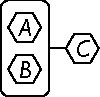
\includegraphics[scale=1]{hex-AparBtnC.pdf}}\end{center}

\noindent For example, this sequent
\[ \vdash \bot\tn\bot, \bot\tn\bot, \bot\tn\bot, \bot\tn\bot, 1, \{[(1\parr 1\parr 1)\tn(1\parr 1\parr 1)]\parr 1\parr (\bot\tn\bot\tn\bot)\parr 1\}\tn\bot \]
could be drawn like this:
\begin{center}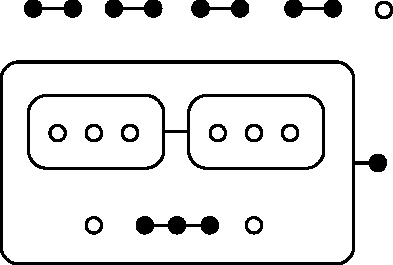
\includegraphics[scale=0.75]{example-sequent.pdf}\end{center}

\noindent We represent a proof net by drawing an arrow from each $\bullet$ to some $\circ$. For example, one proof net on the above sequent is
\begin{center}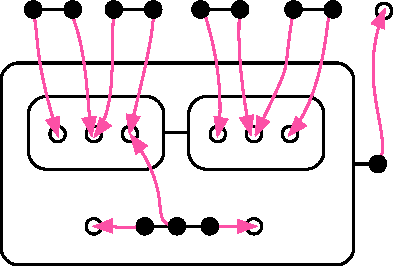
\includegraphics[scale=0.75]{example-sequent-proofnet.pdf}\end{center}





%NOTE: need 'octopus' terminology here

%NOTE: will we need to count arms often enough to make it worthwile to write $|\Gamma|_\bot$ for the number of $\bot$-occurrences in a sequent $\Gamma$?



%------------------------------------------------------------

\section{Equivalence in the absence of $~\protect\parr$}





Let a \emph{1-alternation} sequent be one over formulae of the form $1$ or $\bot\tn\ldots\tn\bot$, where the number of $\bot$-subformulae is at least 2.
%
Such a sequent is inhabited exactly when the number of formulae in the sequent is one greater than the total number of $\bot$-subformulae it contains.
%
An inhabited 1-alternation sequent with only one tensor-formula, i.e.\ a sequent of the form $\1,\ldots,\1,\bot\tn\ldots\tn\bot$ with $n$ $\bot$-subformulae and $n$ $1$-subformulae, will admit $n!$ different proof nets, each with $n$ links.
%
Since no link can re-attach, its equivalence classes are singletons.



\begin{proposition}
\label{prop:level0 max binary}
%
For a 1-alternation sequent with at least two tensor-formulae there are at most two equivalence classes of proof nets.
%
\end{proposition}


%
%\begin{figure}[p]
%\[
%\begin{array}{ccc}
%	\netA 1213 & \perm	& \netA 3213 \\ \\[-6pt] \vperm && \vperm \\ \\[-6pt]
%	\netA 1223 &		& \netA 3212 \\ \\[-6pt] \vperm && \vperm \\ \\[-6pt]
%	\netA 1323 &		& \netA 3112 \\ \\[-6pt] \vperm && \vperm \\ \\[-6pt]
%	\netA 1321 &		& \netA 3132 \\ \\[-6pt] \vperm && \vperm \\ \\[-6pt]
%	\netA 2321 &		& \netA 2132 \\ \\[-6pt] \vperm && \vperm \\ \\[-6pt]
%	\netA 2331 & \perm	& \netA 2131
%\end{array}
%\qquad
%\begin{array}{ccc}
%	\netA 1312 & \perm	& \netA 1332 \\ \\[-6pt] \vperm && \vperm \\ \\[-6pt]
%	\netA 2312 &		& \netA 1232 \\ \\[-6pt] \vperm && \vperm \\ \\[-6pt]
%	\netA 2313 &		& \netA 1231 \\ \\[-6pt] \vperm && \vperm \\ \\[-6pt]
%	\netA 2113 &		& \netA 3231 \\ \\[-6pt] \vperm && \vperm \\ \\[-6pt]
%	\netA 2123 &		& \netA 3221 \\ \\[-6pt] \vperm && \vperm \\ \\[-6pt]
%	\netA 3123 & \perm	& \netA 3121
%\end{array}
%\]
%\caption{The two equivalence classes of nets for $\1,\1,\1,\bot\tn\bot,\bot\tn,\bot$}
%\label{fig:2x12 nets}
%\end{figure}



\begin{IEEEproof}
%
It will be shown by induction on the number of $\bot$-formulae in $\Gamma$ that every proof net for $\Gamma$ belongs to one of two equivalence classes.
%
For the base case, the smallest inhabited sequent with two tensor-formulae is the following.
\[
	\1,\1,\1,\bot\tn\bot,\bot\tn,\bot
\]
It has two equivalence classes, of 12 proof nets each.
%
(Apart from listing these exhaustively, this can also be shown by using the proof of the inductive step, below, to reduce the base case to that of the sequent $\1,\1,\bot\tn\bot$, which has two singleton equivalence classes.)

%, displayed in Figure~\ref{fig:2x12 nets}.



For the inductive step, let $\Gamma$ be the following sequent.
\[
	\Delta,A\tn\named a\bot,\named z\1
\]
There are two cases: 1) where $A$ is a tensor-formula, and 2) where $A$ is $\bot$ and where, for the induction hypothesis to apply, $\Delta$ contains at least two tensor-formulae.
%
For both cases, it will be shown that any net $\links$ for $\Gamma$ is equivalent to a net $\links'$ where $\named a\bot$ connects to $\named z1$, and is the only link to do so.
%
This reduces equivalence on $\Gamma$ to equivalence on $\Delta,A$ in case 1, and on $\Delta$ in case 2, so that the induction hypothesis applies.


In constructing $\links'$, since the proof net must be connected, there is a path from $a$ to $z$.
%
We will consider only the jumps on this path, not any other edges.
%
There are four cases.

\begin{enumerate}
	\item
The path consists of exactly the jump $\edge az$.
%
Let $\edge by$ be a jump from a $\named b\bot$ in $A$; then $\links'$ is obtained from $\links$ by changing: $\links'(e)=y$  for every $\named e\bot$ such that $\links(e)=z$ and $e\neq a$.


	\item
The path starts with the jump $\edge ax$ (and $x\neq z$).
%
Let $\edge by$ be a jump from a $\named b\bot$ in $A$, and let the path end with the jumps $\edge wc$ and $\edge dz$, where $\named c\bot$ and $\named d\bot$ are in the same tensor-formula $B$.
%
Then $\links'$ is obtained from $\links$ by changing: $\links'(a)=z$, and $\links'(e)=w$ for every $\named e\bot$ such that $\links(e)=z$ and $e\neq a$, including $d$.
%
These changes are illustrated as permutations below.
%
\[
	\netB xywz \perm \netB zywz \perm \netB zywy
\]



	\item
The path consists of exactly one jump $\edge bz$ from a $\named b\bot$ in $A$ (and $b\neq a$).
%
Let $\links(a)=y$.
%
Choose a jump $\edge cw$ from $\named c\bot$ in $A$ such that there is another $\edge dw$ from $\named d\bot$ in a formula $B$ (not excluding the possibilities $c=b$ and $c=a$).
%
Let $\edge ex$ be a further jump from $\named e\bot$ in $B$.
%
Then $\links'$ is obtained from $\links$ by changing: $\links'(a)=z$, $\links'(d)=x$, $\links'(e)=y$, and $\links'(f)=x$ for each $f$ (including $b$) such that $\links(f)=z$ and $f\neq a$.
%
These changes are exhibited as a series of permutations below, from top left to bottom left (note that the jump from $d$ moves twice).
%
\[
\begin{array}{ccccc}
	\netC yzwx & \perm & \netC yzzx & \perm & \netC yxzx
	\\ &&&& \vperm \\
	\netC zxxy & \perm & \netC zxzy & \perm & \netC yxzy
\end{array}
\]



	\item
The path starts with a jump $\edge bx$ from a $\named b\bot$ in $A$ (and $b\neq a$, $x\neq z$).
%
Let the path end with the jumps $\edge wc$ and $\edge dz$, and let $\links(a)=y$.
%
Then $\links'$ is obtained from $\links$ by changing: $\links'(c)=y$, $\links'(a)=z$, and $\links'(e)=w$ for every $\named e\bot$ such that $e\neq a$ and $\links(e)=z$, including $d$.
%
This is illustrated below.
\end{enumerate}
%
\[
	\kern-1pt \netB yxwz \perm \netB yxyz \perm \netB zxyz \perm \netB zxyw \kern-1pt 
\]
%
\end{IEEEproof}




\begin{proposition}
\label{prop:level0 may-connect path}
%
For a proof net for a 1-alternation sequent containing a link $\edge{\named a\bot}{\named b\1}$ and a formula $\named c\1$, the following are equivalent.
%
\begin{itemize}
	\item
The edge $\edge ab$ can be permuted to $\edge ac$.
	\item
There is a path from $b$ to $c$ not passing through $a$.
	\item
The path from $a$ to $c$ starts with the jump $a-b$.
\end{itemize} 
\end{proposition}


If a link $\edge ab$ may be reconnected as $\edge ac$ it is said that $a$ \emph{may connect to} $c$. 
%
By the above proposition, it is immediate that if $a$ and $b$ may both connect to $c$, then after actually reconnecting $\edge ac$, still $b$ may connect to $c$.



Consider the following naming scheme for the units in a 1-alternation sequent $\Gamma$ with tensor-formulae $A_1,\dotsc,A_n$.
%
\begin{itemize}

	\item
One $\1$ in $\Gamma$ is named $*$, and the remaining ones with the numbers $n+1,\dotsc,m$.

	\item
A $\bot$-formula in $A_i$ is named by a pair $(i,k)$, where $k=i$ for the first $\bot$-formula in each $A_i$, and for the remaining $\bot$-formulae in all $A_i$, each $k$ is a distinct number in $n+1,\dotsc,m$.

\end{itemize}
%
The naming scheme suggests a linking for $\Gamma$, defined by $\links(i,i)=\star$ and $\links(i,k)=k$ otherwise; i.e\ the first $\bot$ in each tensor-formula connects to $\named *\1$, while other $\bot$-subformulae connect uniquely to the remaining $\1$-subformulae.



A net for $\Gamma$ is interpreted as a combinatorial permutation (an automorphism on $\{1,\dotsc,m\}$) as follows.
%
\begin{definition}
\label{def:combinatorial permutation}
To a proof net $\links$ for a 1-alternation sequent $\Gamma$ named as above, associate the \emph{permutation} $\prm:\{1,\dotsc,m\}\to\{1,\dotsc,m\}$ given by:
\[
	\prm(k) = 
	\begin{cases}
		i				& \text{ if $(i,k)$ may connect to $*$; and}
	\\	\links(i,k)		& \text{ otherwise.}
	\end{cases}
\]
The \emph{parity} of $\links$ is the parity of its permutation.
\end{definition}


To see that $\prm$ is injective, consider the following.
\begin{itemize}
	\item The domains of $i$ and $\links(i,k)$, respectively $1,\dotsc,n$ and $n+1,\dotsc,m$, are disjoint.
	\item Exactly one $\bot$-formula in each $A_i$ may connect to $*$ because of connectedness and acyclicity, since if a $\bot$-formula may connect to $*$ it has a path to $*$ (Proposition~\ref{prop:level0 may-connect path}).
	\item If two $\bot$-formulae have the same target, which means they are in different tensor-formulae, at least one may connect to $*$ via the other tensor-formula, which must have a path to $*$ by the above.
\end{itemize}



\begin{proposition}
\label{prop:level0 min binary}
A permutation on a net $\links$ preserves its parity. 
\end{proposition}


\begin{IEEEproof}
Let $\links$ be a net for $\Gamma$, with $\Gamma$ named as above, and let the link $\edge{(i,k)}x$ in $\links$ re-attach as $\edge{(i,k)}y$, forming $\links'$.
%
There are two cases, depending on whether $(i,k)$ may connect to $*$.
%
If so, using Proposition~\ref{prop:level0 may-connect path}, the re-wiring preserves which $\bot$-formulae may connect to $*$, since for any path to $*$ via $\edge{(i,k)}x$ in $\links$ there is a path to $*$ via $\edge{(i,k)}y$.
%
Then the permutation of $\links'$ is that of $\links$.


If $(i,k)$ may not connect to $*$, let the path from $x$ to $y$ run via the following $\bot$- and $\1$-vertices.
\[
	x=x_1, (i_1,j_1), (i_1,k_1), x_2, (i_2,j_2), \dotsc, (i_n,k_n), x_{n+1}=y 	
\]
Note that the $\bot$-formulae $(i_a,j_a)$ may connect to $*$.
%
On the relevant domain, this gives the following permutation for $\links$.
\[
\left(\begin{array}{ccccccc}
	j_1 & \dotso & j_n &  k  & k_1 & \dotso & k_n \\
	i_1 & \dotso & i_n & x_1 & x_2 & \dotso & x_{n+1}
\end{array}\right)
\]
In $\links'$, since $\links'(i,k)=y$, the $\bot$-formulae that may connect to $*$ are the $(i_a,k_a)$.
%
The permutation $\prm[\links']$ is the following.
\[
\left(\begin{array}{ccccccc}
	j_1 & \dotso & j_n &    k    & k_1 & \dotso & k_n \\
	x_1 & \dotso & x_n & x_{n+1} & i_1 & \dotso & i_n
\end{array}\right)
\]
The parity of both permutations is the same if and only if the relative permutation, below, is even.
\[
\left(\begin{array}{ccccccc}
	i_1 & \dotso & i_n & x_1     & x_2 & \dotso & x_{n+1} \\
	x_1 & \dotso & x_n & x_{n+1} & i_1 & \dotso & i_n
\end{array}\right)
\]
This is the case, as it is obtained by the exchange of $x_a$ and $i_a$ for each $a\leq n$, and subsequently the exchange of $x_{n+1}$ and each $i_a$ in turn.
%
\end{IEEEproof}



\begin{proposition}
\label{prop:parity determines equivalence}
Two proof nets for a 1-alternation sequent with at least two tensor-formulae are equivalent if and only if they have the same parity.
\end{proposition}


\begin{theorem}
\MLL\ proof equivalence in the absence of ~$\parr$ is linear-time decidable.
\end{theorem}

\begin{IEEEproof}
For a sequent with 1 tensor-formula, the problem is reduced to syntactic equality.
%
For a sequent with 2 or more tensor-formulae, by Propositions~\ref{prop:parity determines equivalence} the equivalence of two nets is determined by their parity.
%
Following Definition~\ref{def:combinatorial permutation} the parity of a net can be read off in a single traversal of the net.
%
This yields a linear-time algorithm.
%
\end{IEEEproof}




\begin{lemma}
\label{lem:double exchange}
Let $\links$ be a proof net where $\links(a)=(u)$, $\links(b)=v$, $\links(c)=x$, and $\links(d)=y$, and for any switching the path from $u$ to $y$ passes through the links $b-v$ and $x-c$.
%
Then $\links\sim\links'$ where $\links'(a)=v$, $\links'(b)=u$, $\links'(c)=y$, and $\links'(d)=x$, and $\links'(z)=\links(z)$ otherwise.
\end{lemma}

\begin{IEEEproof}
\[
	\vc{\doubleExchange uvxy}
	\sim
	\vc{\doubleExchange uyxy}
	\sim
	\vc{\doubleExchange uyxu}
	\sim
	\vc{\doubleExchange vyxu}
	\sim
	\vc{\doubleExchange vyyu}
	\sim
	\vc{\doubleExchange vuyu}
	\sim
	\vc{\doubleExchange vuyx}
\]
\end{IEEEproof}



%------------------------------------------------------------


\section{Par}



\begin{definition}
A \emph{sub-sequent} $\Delta\leq\Gamma$ of a sequent $\Gamma$ is a sequent consisting of disjoint subformulae of $\Gamma$, preserving names.
\end{definition}


\begin{definition}
A \emph{subnet} $(\Gamma',\links') \leq (\Gamma,\links)$ of a proof net is a net such that $\Gamma'\leq\Gamma$ and $\links'$ is $(\links|_{\Gamma'})$, the restriction of $\links$ to $\Gamma'$.
\end{definition}


The root vertices of $\Gamma'$ are the \emph{ports} of the sub-sequent $\Gamma'$ and of the subnet $(\Gamma',\links')$.
%
A \emph{scope} of a par $\named v\parr$ is a subnet that has $v$ as a port.
%
In a proof net, the \emph{kingdom} and the \emph{empire} of a par are respectively its smallest and largest scope.



The scopes of a par correspond to the possible subproofs of its introduction rule in a sequentialisation of the proof net that it occurs in.
%
In the graph of a proof net, the scope of a par $\named v\parr$ may be \emph{contracted} to a single vertex $v$ by removing all vertices except $v$ and re-attaching all arcs connecting to removed vertices to $v$.
%

[[ ADD ILLUSTRATED EXAMPLE ]]

%
The contraction of scopes may replace the switching condition as a correctness criterion.
%
The following is a variant of the local retraction algorithm by Danos \cite{Danos-1990}.


\begin{proposition}
\label{prop:scoping correctness}
A linking $\links$ for a sequent $\Gamma$ is a proof net if and only if each $\named v\parr$ is a port of a sub-sequent $s(v)\leq\Gamma$ such that:

\begin{enumerate}
	\item
sub-sequents are strictly nested: if $\named w\parr$ occurs in $s(v)$ then $s(w)<s(v)$; and
	\item
for each $\named v\parr$, the graph $\sigma(v)=(s(v),\links|_{s(v)})$ becomes a tree when all immediate sub-sequents $s(w)$ are contracted.
\end{enumerate}

\end{proposition}


\begin{IEEEproof}
For the `if' direction, it follows by induction on the nesting of sub-sequents that each graph $\sigma(v)$ satisfies the switching condition.
%
For the `only if' direction, given a sequentialisation of $(\Gamma,\links)$, a sub-sequent $s(v)\leq\Gamma$ for each $\named v\parr$ is found by taking the conclusion $\Delta, A\named v\parr B$ of its introduction rule, below.
\[
	\infer{\Delta,A\named v\parr B}{\Delta,A,B}
\]
\end{IEEEproof}





[[ IDEA: the following could help simplify octopus-arithmetic ]]


\begin{definition}
The \emph{balance} of a sequent is the number of $\bot$s minus the number of $\parr$s and comma's.
%
A sequent is \emph{balanced} if its balance is zero.
\end{definition}

An unbalanced sequent is uninhabited: a positive balance guarantees a cycle in any switching graph, for any linking, while a negative balance similarly guarantees disconnectedness.

An early conjecture of Girard, which turned out to be false, was that a sequent is inhabited if and only if it is balanced. [[FIND CITATION (probably TCS87)]]








%------------------------------------------------------------


\section{Proof nets and constraint graphs}



[[ NOTE: we should decide on notation for steps versus paths in permutation relations ]]



\begin{definition} 
A \emph{non-deterministic constraint graph} (\textsc{ncg}) $G=(V,E,c,v,w)$ consists of a set $V$ of vertices with \emph{minimum inflow constraint} $c\colon V\to\mathbb N$, and a set $E$ of at most one undirected edge $e$ per vertex-pair $v(e)=\{v_1,v_2\}$, with \emph{weight} $w\colon E\to N$.

A (partial) \emph{configuration} of an \textsc{ncg} is a (partial) function $\gamma\colon E\to V$ such that
\begin{itemize}
	\item
for every edge $e$, $\gamma(e)\in v(e)$ or (in the partial case) $\gamma(e)$ is undefined, and
	\item
for every vertex $v$, the sum of its inflow weights is at least its inflow constraint, $\sum\{w(e)\mid \gamma(e)=v\}\geq c(v)$.
\end{itemize} 

A \emph{reconfiguration step} $\gamma\sim\delta$ connects two (partial) configurations for an \textsc{ncg} $G$ that differ in the assignment of exactly one edge.

\end{definition}


The \emph{(partial) \textsc{ncg}-reconfiguration problem} is the problem of deciding when two (partial) configurations are connected by a path in the graph of (partial) configurations and reconfiguration steps.

\begin{theorem}[\cite{demaine}]
\textsc{ncg}-reconfiguration is \textsc{pspace}-complete.
\end{theorem}

\begin{proposition}
Partial \textsc{ncg}-reconfiguration is \textsc{pspace}-complete.
\end{proposition}

\begin{IEEEproof}
There is a path between total configurations $\gamma$ and $\delta$ in partial \textsc{ncg}-reconfiguration if and only if there is one in \textsc{ncg}-reconfiguration, for the following two reasons.
%
Firstly, if $\gamma\sim\delta$ are partial configurations, they may be completed to total configurations $\gamma'\sim\delta'$ or $\gamma'=\delta'$.
%
Secondly, if $\gamma'$ and $\gamma''$ are total configurations that both agree with a partial configuration $\gamma$ where it is defined, then $\gamma'$ and $\gamma''$ are connected in \textsc{ncg}-reconfiguration by re-assigning the values where they disagree.
%
\end{IEEEproof}


For a graph $G=(V,E,c,v,w)$ let $|V|$ and $|E|$ denote the number of vertices and edges, respectively, and let $|c|$ and $|w|$ denote the sum of all inflow constraints, $\sum_{v\in V}c(v)$, and the sum of all edge weights, $\sum_{e\in E}w(e)$.


Let $A^n$ denote the sequent of $n$ copies of a formula $A$, and for a sequent $\Gamma=A_1,\dotsc,A_n$ let $\bigotimes\Gamma=A_1\tn\dotso\tn A_n$ and $\bigparr\Gamma=A_1\parr\dotso\parr A_n$.



\begin{definition}
\label{def:graph interpretation}
The \emph{interpretation} $\itn G$ of an \textsc{ncg} $G=(V,E,c,v,w)$ is a sequent constructed as follows.
%
Let $V=\{v_1,\dotsc,v_n\}$ and $E=\{e_1,\dotsc,e_m\}$ where $|V|=n$ and $|E|=m$.

The interpretation of a vertex $v_k$ is the formula
\[
	\itn{v_k} = \bigparr\big(C^{m\times c(v_k)} \big)\parr 1
\]
where each \emph{constraint element} $C$ is the formula
\[
	C = \bigparr\big(1^{3k+2}\big) \tn \bigparr\big(1^{3(n-k)+3}\big)
\]

The interpretation of an edge $e$ connecting vertices $v_i$ and $v_j$ with $i<j$ is the formula
\[
	\itn{e} = \bigotimes\big(W^{m\times w(e)}\big)\tn\bot
\]
where each \emph{weight element} $W$ is the formula
\[
	W = \bigotimes\big(\bot^{3i+2}\big)\parr\bigotimes\big(\bot^{3(j-i)+1}\big)\parr\bigotimes\big(\bot^{3(n-j)+3}\big)
\]

The interpretation of the graph $G$ is the sequent
\[
	%\itn G = \bigotimes_{1\leq i\leq n}\itn{v_i}, \itn{e_1},\dotsc,\itn{e_k}, \bot^m
	\itn G = \itn{v_1}\tn\dotso\tn\itn{v_n}, \itn{e_1},\dotsc,\itn{e_m}, 1^p
\]
where $p=m\times(|w|-|c|)\times(3n+4)$; the $p$ instances of $1$ are called \emph{edge-absorbers}.

\end{definition}



In an \textsc{ncg} $G$, a vertex $v$ and an edge $e$ will be called \emph{appropriate} (for each other) if $v\in v(e)$, and \emph{inappropriate} otherwise.
%
This notion is extended to vertex-gadgets $\itn v$ and edge-gadgets $\itn e$ in $\itn G$.



For a weight element $W$ of an edge connecting $v_i$ and $v_j$, let the $\bot$-occurrences be named as follows,
\[
	W =  \big(\named{    \dagger}\bot\tn\named{   1}\bot\tn\dotsc\tn\named{3i+1}\bot\big)
	\parr\big(\named{   \ddagger}\bot\tn\named{3i+2}\bot\tn\dotsc\tn\named{3j+1}\bot\big)
	\parr\big(\named{\downdagger}\bot\tn\named{3j+2}\bot\tn\dotsc\tn\named{3n+3}\bot\big)
\]
and the $1$-occurrences of a constraint element $C$ in $\itn{v_k}$,
\[
	C = \big(\named{\alt    \dagger}1\parr\named{\alt{   1}}1\parr\dotso\parr\named{\alt{3k+1}}1\big)
	\tn \big(\named{\alt\downdagger}1\parr\named{\alt{3k+2}}1\parr\dotso\parr\named{\alt{3n+3}}1\big)~.
\]
There is a \emph{natural linking} for the sequent $W,C$ if $e$ is appropriate for $v_k$, i.e.\ if $k=i$ or $k=j$, as follows:
\[
	\links(x) = \alt x \qquad \text{for }x\in\{\dagger,\downdagger\}\cup\mathbb N
\]
\[
	\links(\ddagger)=
	\begin{cases}
		\alt	\dagger & \text{if }k=i \\
		\alt\downdagger & \text{if }k=j~.
	\end{cases}
\]
There is also a natural linking for the sequent $W,\named\star 1,\named{\alt 1}1,\dotsc,\named{\alt {3n+3}}1$ consisting of the weight element $W$ and $3n+4$ edge-absorbers:
\[
	\links(x)=
	\begin{cases}
		\star  & \text{if }x\in\{\dagger,\ddagger,\downdagger\} \\
		\alt x & \text{otherwise }.
	\end{cases}
\]


\begin{proposition}
\label{prop:element linkings}
\begin{enumerate}
	\item
Given a vertex $v$ and an appropriate edge $e$, for a constraint element $C$ in $\itn v$ and a weight element $W$ in $\itn e$ the natural linking for the sequent $W,C$ is a proof net.
	\item
Given a weight element $W$ for a graph with $|V|=n$, the natural linking for the sequent $W,1^{3n+4}$ is a proof net.
\end{enumerate}
\end{proposition}


The rightmost $1$-occurrence of each vertex-gadget $\itn v$, named $\alt v$ below, and the rightmost $\bot$-occurrence of each edge-gadget $\itn e$, named $\alt e$, will be called the \emph{indicator vertices} of $\itn v$ and $\itn e$.
\[	
	\itn v = C\parr\dotso\parr C\parr \named{\alt v}1 \qquad \itn e= W\tn\dotso\tn W\tn\named{\alt e}\bot~.
\]


\begin{definition}
\label{def:configuration interpretation}
The \emph{interpretation} $\itn\gamma$ of a total configuration $\gamma$ for a graph $G$ is a linking $\links$ constructed incrementally, for each successive edge $e$, and for each successive weight element $W$ within $e$, as follows.
%
Let $\gamma(e)=v$; firstly, the the indicator vertex of $\itn e$ links to the indicator of $\itn v$.
%
Then successively for each weight element $W$ in $e$, if $\itn v$ has a first free constraint element $C$, extend $\itn\gamma$ to include the natural linking on $W,C$; otherwise, extend $\itn\gamma$ by the natural linking on the sequent consisting of $W$ plus the first $3n+4$ free edge absorbers.
\end{definition}


\begin{proposition}
If $\gamma$ is a total configuration for $G$ then $\itn\gamma$ is a proof net for $\itn G$.
\end{proposition}

\begin{IEEEproof}
Using Proposition~\ref{prop:scoping correctness}, it is sufficient to give a suitable scope for each $\parr$. 
%
The scope of each weight element $W$ is the sequent $W,C$ or $W,1^{3n+4}$ of its natural linking, which forms a proof net by Proposition~\ref{prop:element linkings}.
%
The scope of each vertex-gadget $\itn v$ contains the edge-gadgets $\itn e$ such that $\gamma(e)=v$, plus all the edge-absorbers within scopes of weight elements inside $\itn e$.
%
Since the weights of the connected edges $e$ sum to more than the inflow constraint of $v$, there are no unused constraint elements remaining in $\itn v$.
%
After contracting the scope of each $W$, each edge-gadget in the scope of $\itn v$ becomes a single string of connected vertices, connected to other edge-gadgets only via the special $\named v1$ of $\itn v$, thus forming a tree.
\end{IEEEproof}



% - - - - - - - - - - - - - - - - - - - - - - - - - - - - - -

\subsection*{Completeness}


In a proof net for $\itn G$, an edge-gadget $\itn e$ that is in the empire of an appropriate vertex-gadget $\itn v$ is \emph{naturally linked} if the indicator of $\itn e$ connects to the indicator of $\itn v$, and each weight element $W$ of $\itn e$ is either naturally linked to a constraint element $C$ in $\itn v$ or linked only to edge-absorbers.

\begin{lemma}
\label{lem:octopus roll}
In a proof net $\links$ for a sequent $\Gamma=\itn v,\itn{e_1},\dotsc,\itn{e_m},\bot^p$ where each edge-gadget is naturally linked, if a weight element $W_i$ in $\itn{e_i}$ is linked to $C$ in $\itn v$ and $W_j$ in $\itn{e_j}$ is linked to edge-absorbers $\bot^n$, then there is a net $\links'\sim\links$ in which $W_j$ is naturally linked to $C$, $W_i$ is linked to $\bot^n$, and $\links'$ agrees with $\links$ otherwise.
\end{lemma}

\begin{IEEEproof}
Let $W_i=A\parr B\parr C$, $W_j=D\parr E\parr F$, and $C=X\tn Y$.
%
We will illustrate the path of permutations for the case where $A,B,X$ and $D,X$, and thus also $C,Y$ and $E,F,Y$, are balanced sequents; other cases are similar.
%
\begin{enumerate}
	\item
The initial configuration is illustrated below; other weight and constraint elements are omitted, and $v$, $i$, and $j$ are the indicator vertices of $\itn v$, $\itn{e_i}$, and $\itn{e_j}$ respectively.
\[
	\octorollA1
\]
	\item
The link $i-v$ is re-attached to connect to an edge-absorber together with only the links from the first $\bot$ of each of $D$, $E$, and $F$. 
\[
	\octorollB2
\]
	\item
Secondly, the link from the first $\bot$ of $D$ is moved to $X$, and those of $E$ and $F$ are moved to $Y$.
\[
	\octorollB3
\]
	\item\label{item:exchange added}
There are subnets over the sub-sequents $A,B,X,D,\bot^m$ and $C,Y,E,F,\bot^k$.
%
These subnets may be rewired so that $D\parr E\parr F$ is naturally linked to $X\tn Y$: by Proposition~\ref{prop:parity determines equivalence}, the resulting subnets are equivalent as long as their parity is preserved.
%
Two links from $C$ to $X$ should remain exchanged, compared to the natural linking, for step \ref{item:exchange needed} below.
%
The links of $A,B,C$ connect to the edge-absorbers $\bot^m$ and $\bot^k$, with one remaining link from $B$ to $X$ and one from $C$ to $Y$.
\[
	\octorollC
\]
	\item
The link from $C$ to $Y$ is moved towards an edge-absorber connected to $A,B$.
\[
	\octorollD1
\]
	\item\label{item:exchange needed}
The link from $B$ to $X$ is the one remaining connection between the edge-gadgets $\itn{e_i}$ and $\itn{e_j}$.
%
Lemma~\ref{lem:double exchange} allows to swap the targets of the link from $B$ to $X$ and the link from $i$, and simultaneously undo the exchange in the links from $C$ to $X$ added in step \ref{item:exchange added} above.
\[
	\octorollD2
\]
	\item
The link from $i$ may be re-attached to $v$ to yield the final configuration.
\[
	\octorollA2
\]
\end{enumerate}
\end{IEEEproof}


An edge-gadget $\itn e$ is \emph{free} if each of its weight elements is linked only to edge-absorbers.


\begin{lemma}
\label{lem:permute edge-absorbers}
If $\links$ is a naturally linked proof net for $\itn G$ with a free edge-gadget $\itn e$, and $\links'$ agrees with $\links$ up to an even permutation of edge-absorbers, then $\links\sim\links'$.
\end{lemma}

\begin{IEEEproof}
Let $e_0$ be the indicator vertex of $\itn e$; since $\itn e$ is free, $e_0$ may re-attach anywhere within the proof net.
%
Let $e_1$ and $e_2$ be arbitrary other $\bot$-occurrences in $\itn e$.

\begin{enumerate}

	\item
To permute two edge-absorbers $v$ and $w$ linked to by other edge-gadgets than $\itn e$, attach $e_0$ to $v$, and apply Lemma~\ref{lem:double exchange} to exchange $v$ and $w$, also exchanging the targets of $e_0$ and $e_1$.

	\item
To reinstate $e_0$ as the connection between $\itn e$ and the remainder of the proof net, either perform another permutation as above, or permute $v$ and $w$ twice again, once exchanging the targets of $e_1$ and $e_2$, and once exchanging the targets of $e_2$ and $e_0$.

	\item
To exchange an edge-absorber $w$ linked from a $\named d\bot$ outside $\itn e$ for the target $v$ of $e_1$, and attach $e_0$ to $w$, attach $d$ to $v$.
%
At this point, $e_1$ forms the only connect between $\itn e$ and the remainder of the proof net; to reinstate $e_0$ in this role, do as above, producing a net effect of cycling the targets of $e_1$, $e_2$, and $d$.

	\item
Finally, to permute edge-absorbers $v$ and $w$ linked by $\itn e$, attach $e_0$ to the indicator of a vertex-gadget where also another edge-gadget $\itn d$ is connected, with indicator vertex $d_0$ and an arbitrary other vertex $d_1$.
%
Connect $d_0$ to $v$, and apply Lemma~\ref{lem:double exchange} to permute $v$ and $w$, as well as exchanging the targets of $d_0$ and $d_1$.
%
A second such exchange is needed to re-attach $d_0$ and $d_1$ to their original targets.

\end{enumerate}

In each case, if one of the edge-absorbers exchanged is linked to by multiple $\bot$-occurrences within the same weight element, these may be termporarily attached elsewhere.

\end{IEEEproof}

Let $\itn\gamma'$ be $\itn\gamma$ where the first two edge-absorbers are exchanged.

\begin{lemma}
If $\gamma\sim\delta$ for total configurations $\gamma$ and $\delta$, then either $\itn\gamma\sim\itn\delta$ or $\itn\gamma\sim\itn\delta'$.
\end{lemma}

\begin{IEEEproof}
We will prove the case where $\gamma\sim\delta$ is a single reconfiguration step; the general case follows because the proof goes through also when $\itn\gamma'$ replaces $\itn\gamma$ in the statement of the lemma.
%
Let $\gamma$ and $\delta$ agree on every edge except $e$, where $\gamma(e)=v$ and $\delta(e)=w$.
%
Firstly, using Lemma~\ref{lem:octopus roll}, for the edges $d$ other than $e$ such that $\gamma(d)=v$, the weight elements of the edge-gadgets $\itn d$ may be linked to the constraint elements of $\itn v$, in accordance with the target configuration $\itn\delta$.
%
Since $e$ is mobile in $\gamma$, the weights of the edges $d$ suffice to fill the inflow constraint of $v$, and correspondingly the weight elements of edge-gadgets $\itn d$ suffice to fill the constraint elements of $\itn v$, so that $\itn e$ is free.
%
Next, the indicator vertex of $\itn e$, which links to the indicator of $\itn v$, is re-attached to the indicator of $\itn w$.
%
Again using Lemma~\ref{lem:octopus roll}, the weight elements of edge-gadgets connected to $\itn w$, including $\itn e$, may be linked in accordance with $\itn\delta$.
%
The resulting proof net is $\itn\delta$ modulo a permutation of edge-absorbers; then it is equivalent to either $\itn\delta$ or $\itn\delta'$ by Lemma~\ref{lem:permute edge-absorbers}.
\end{IEEEproof}


% - - - - - - - - - - - - - - - - - - - - - - - - - - - - - -

\subsection*{Soundness}


\begin{lemma}
In a proof net for $\itn G$, an edge-gadget $\itn e$ belongs to the empire of at most one vertex-gadget $\itn v$.
\end{lemma}

\begin{IEEEproof}
Since vertex-gadgets are joined by a tensor, the lemma is immediate from \cite[Proposition 1]{Bellin-vandeWiele-1995}.
\end{IEEEproof}




\begin{lemma}
\label{lem:appropriate edge weights}
In a proof net for $\itn G$, for each vertex $v$, the weights of the appropriate edge-gadgets in the empire of $\itn v$ are equal to or greater than the constraint of $v$.
\end{lemma}


\begin{IEEEproof}
Let $|V|=n$ and $|E|=m$, and consider the vertex $v_i$ and an edge $e$ connecting vertices $v_a$ and $v_b$ where $i\neq a,b$.
%
Each constraint element in $\itn{v_i}$ is an instance of the formula
\[
	C = \bigparr\big(1^{3i+2}\big) \tn \bigparr\big(1^{3(n-i)+3}\big)~.
\]
The two $\parr$-subformulae have a balance of $-3i-1$ and $-3(n-i)-2$ respectively.
%
Each weight element in $\itn{e}$ is an instance of 
\[
	W = \bigotimes\big(\bot^{3a+2}\big)\parr\bigotimes\big(\bot^{3(b-a)+1}\big)\parr\bigotimes\big(\bot^{3(n-b)+3}\big)~.
\]
The three $\tn$-subformulae have a net balance of $3a+1$, $3(b-a)$, and $3(n-b)+2$ respectively.
%
In pairs, they have a net balance of $3b+1$ (1st and 2nd subformula), $3(a+n-b)+3$ (1st and 3rd), and $3(n-a)+2$ (2nd and 3rd).
%
Since $i\neq a,b$, and since no $\tn$-subformula of $W$ can connect to more than one $\parr$-subformula of $C$, it follows that $W$ can balance the scope of at most one of both subformulae of $C$.


The vertex-gadget $\itn{v_i}$ is the formula
\[
	\itn{v_i} = \bigparr\big(C^{m\times c(v_i)} \big)\parr 1~.
\]
It will be shown that $m$ inappropriate edge-gadgets may balance at most $m-1$ constraint elements $C$.


Let the root nodes of the two $\parr$-subformulae of each instance of $C$ be labelled $x_j$ and $y_j$, for $1\leq j\leq m\times c(v_i)$. 
%
If the scopes $s(x_j)$ and $s(y_m)$ of any $x_j$ and $y_m$ are balanced by weight elements $W$ and $W'$ of the same edge-gadget $\itn e$, then since $W$ and $W'$ are connected by a tensor, there are switchings of $W$, $W'$, $s(x_j)$, and $s(y_m)$ such that $x_j$ and $y_m$ are connected in the proof net for $\itn G$.
%
Then the first constraint element of $\itn{v_i}$ requires 2 edge-gadgets to balance, and each successive element requires one additional edge-gadget.
\end{IEEEproof}



Using the above, a proof net for $\itn G$ may be interpreted as a configuration for $G$.



\begin{definition}
For a proof net $\links$ for the interpretation of a graph $\itn G$, let $\coitn\links$ be the partial configuration for $G$ where $\coitn\links(e)$ is $v$ if 1) $e$ is appropriate for $v$ and 2) $\itn e$ belongs to the empire of $\itn v$, and undefined otherwise.
\end{definition}



\begin{lemma}
If $\links\sim\links'$ are proof nets for $\itn G$ then $\coitn\links\sim\coitn{\links'}$.
\end{lemma}

\begin{IEEEproof}
A single permutation $\links\sim\links'$ on proof nets may move a number of edge-gadgets $\itn{e_1},\dotso,\itn{e_n}$ in three ways: 1) out of the empire of a vertex-gadget $\int v$, 2) into the empire of a vertex-gadget $\int w$, or 3) both.
%
Then in both $\coitn\links$ and $\coitn{\links'}$ the edges $e_1$ through $e_n$ are mobile, since by Lemma~\ref{lem:appropriate edge weights} the empires of the vertex-gadgets $\itn v$ (in cases 1 and 3) and $\itn w$ (in cases 2 and 3) contain appropriate edge-gadgets other than $\itn{e_1}$ through $\itn{e_n}$ of sufficient combined weight.
%
It follows that in the graph $G$ the edges $e_1$ through $e_n$ can be moved away from $v$ and/or onto $w$ one at a time.

\end{IEEEproof}



%------------------------------------------------------------


\section{Conclusions}








%===========================
\bibliographystyle{plain}
\bibliography{../refs}
\end{document}
%===========================









\end{document}












